% =====================================================================
%  Informe técnico — Proyecto II · Programación III · UNSAAC
%  Sistema de Análisis y Optimización de Redes Financieras (OptiFin Amazonía)
%  Compilar con XeLaTeX:   xelatex informe.tex   (dos veces, para el índice)
% =====================================================================
\documentclass[11pt,a4paper]{article}

% ---------- idioma y fuentes ----------
\usepackage{fontspec}
\usepackage{polyglossia}
\setmainlanguage{spanish}
\setmainfont{TeX Gyre Termes}
\setmonofont{VictorMono}[Path=./fonts/, Extension=.ttf, UprightFont=*-Regular,
  BoldFont=*-Bold, ItalicFont=*-Italic, BoldItalicFont=*-BoldItalic, Scale=0.86]

% ---------- página ----------
\usepackage[a4paper,margin=2.5cm,headheight=14pt]{geometry}
\usepackage{setspace}
\setstretch{1.12}
\renewcommand{\topfraction}{0.95}\renewcommand{\textfraction}{0.05}\setcounter{topnumber}{3}
\setlength{\parindent}{1.27cm}   % sangría APA 7
\setlength{\parskip}{0pt}

\usepackage{fancyhdr}
\pagestyle{fancy}
\fancyhf{}
\fancyhead[L]{\small OptiFin Amazonía — Informe técnico}
\fancyhead[R]{\small\thepage}      % número de página arriba a la derecha (APA 7)
\renewcommand{\headrulewidth}{0.4pt}

% ---------- utilidades ----------
\usepackage{graphicx}
\usepackage{xcolor}
\usepackage{array,tabularx,multirow,makecell}
\usepackage{amsmath,amssymb}
\usepackage{enumitem}
\setlist{itemsep=1pt,topsep=3pt,leftmargin=1.5em}
\usepackage{float}
\usepackage{caption}
\usepackage{listings}
\usepackage{tikz}
\usetikzlibrary{positioning,arrows.meta,shapes.geometric}
\usepackage[hidelinks]{hyperref}
\usepackage{xurl}
\usepackage[round,authoryear]{natbib}
\setlength{\bibsep}{1pt}
\setlength{\bibhang}{1.27cm}    % sangría francesa APA

% ---------- encabezados en formato APA 7 ----------
\usepackage{titlesec}
\titleformat{\section}{\normalfont\large\bfseries\filcenter}{\thesection.}{0.5em}{}
\titleformat{\subsection}{\normalfont\normalsize\bfseries}{\thesubsection}{0.5em}{}
\titleformat{\subsubsection}{\normalfont\normalsize\bfseries\itshape}{\thesubsubsection}{0.5em}{}
\titlespacing*{\section}{0pt}{10pt}{5pt}
\titlespacing*{\subsection}{0pt}{8pt}{3pt}
\titlespacing*{\subsubsection}{0pt}{6pt}{2pt}

% ---------- tablas y figuras en formato APA 7 (número en negrita, título en cursiva, arriba) ----------
\captionsetup{labelsep=newline,justification=raggedright,singlelinecheck=false,
  labelfont=bf,textfont=it,font=small,skip=3pt}
\captionsetup[table]{name=Tabla,position=top}
\captionsetup[figure]{name=Figura,position=top}
\gappto\captionsspanish{\renewcommand{\listtablename}{Índice de tablas}\renewcommand{\contentsname}{Índice}%
  \renewcommand{\listfigurename}{Índice de figuras}\renewcommand{\tablename}{Tabla}}
\emergencystretch=2em
\newcommand{\nota}[1]{\par\vspace{2pt}{\raggedright\footnotesize\textit{Nota.} #1\par}}
% tablas cerradas: todas las celdas con borde
\renewcommand{\arraystretch}{1.18}
\setlength{\arrayrulewidth}{0.5pt}
\newcolumntype{L}[1]{>{\raggedright\arraybackslash}p{#1}}
\newcolumntype{C}[1]{>{\centering\arraybackslash}p{#1}}
\newcolumntype{Y}{>{\raggedright\arraybackslash}X}
\definecolor{cabecera}{HTML}{E2F2EF}
\newcommand{\cab}[1]{\textbf{#1}}
\usepackage[table]{xcolor}

% ---------- código (Victor Mono) ----------
\definecolor{fondo}{HTML}{F6F8FA}
\definecolor{clave}{HTML}{0F766E}
\definecolor{coment}{HTML}{6B7280}
\definecolor{cadena}{HTML}{B45309}
\lstset{basicstyle=\ttfamily\footnotesize, keywordstyle=\color{clave}\bfseries,
  commentstyle=\color{coment}\itshape, stringstyle=\color{cadena}, backgroundcolor=\color{fondo},
  frame=single, rulecolor=\color{gray!50}, numbers=left, numberstyle=\tiny\color{coment},
  xleftmargin=1.6em, framexleftmargin=1.4em, breaklines=true, columns=fullflexible,
  showstringspaces=false, language=Python, morekeywords={self}, aboveskip=4pt, belowskip=2pt}
\renewcommand{\lstlistingname}{Código}

\newcommand{\id}[1]{\texttt{#1}}

\begin{document}

%==================== CARÁTULA ====================
\begin{titlepage}
\thispagestyle{empty}
\begin{center}
\vspace*{0.2cm}
{\Large\bfseries UNIVERSIDAD NACIONAL DE SAN ANTONIO ABAD DEL CUSCO\par}
\vspace{0.5cm}
{\bfseries FACULTAD DE INGENIERÍA ELÉCTRICA, ELECTRÓNICA,\\ INFORMÁTICA Y MECÁNICA\par}
\vspace{0.5cm}
{\bfseries ESCUELA PROFESIONAL DE INGENIERÍA INFORMÁTICA Y DE SISTEMAS\par}
\vspace{0.6cm}
% ---- Logo de la carrera ----
\IfFileExists{logo_carrera_negro.png}{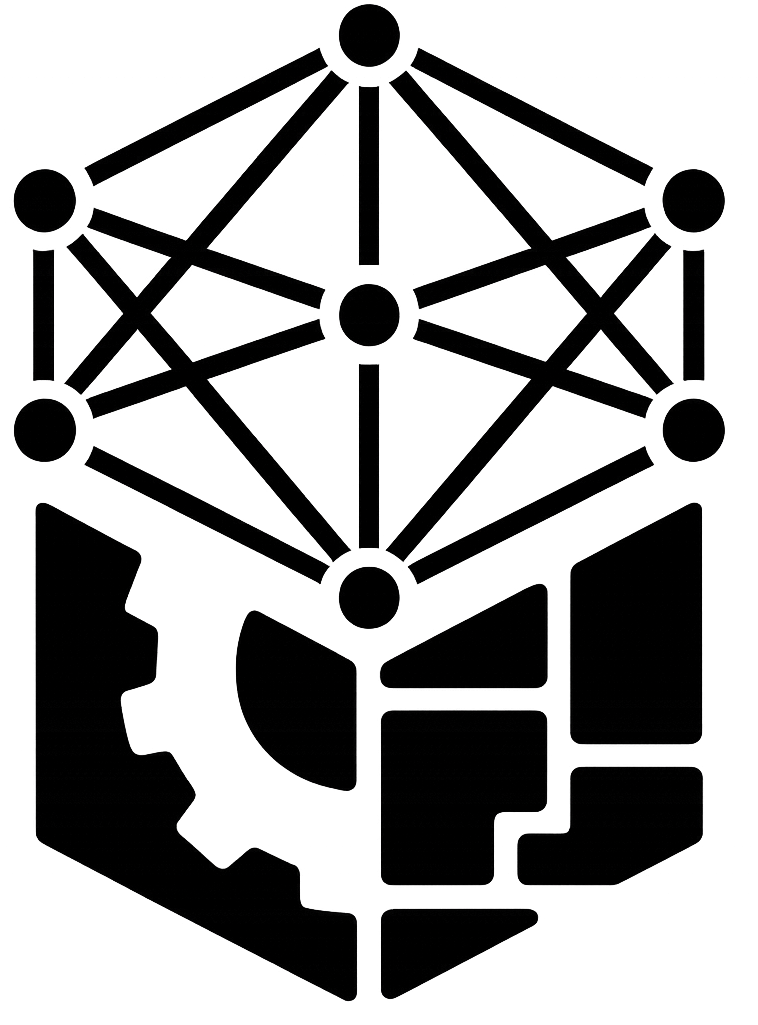
\includegraphics[height=6.5cm]{logo_carrera_negro.png}}{%
  \fbox{\parbox[c][4.8cm][c]{4.8cm}{\centering\small [Aquí va el logo\\ de la carrera]}}}\\[18pt]
{\Huge\bfseries INFORME TÉCNICO\par}
\vspace{0.3cm}
{\Large\bfseries Proyecto II: Sistema de Análisis y Optimización\\ de Redes Financieras\par}
\vspace{0.2cm}
{\large\itshape OptiFin Amazonía\par}
\vspace{0.8cm}
\begin{tabular}{rl}
\large Curso: & \large Programación III\\[6pt]
\large Docente: & \large Karla Catherine Rojas Pedraza\\[6pt]
\large Integrantes: & \large Baca Pauccar, Elmer Leonel\\[2pt]
 & \large Huillca Casa, Erik\\[2pt]
 & \large Quispe Hermoza, Roberto Carlos\\[2pt]
 & \large Quispe Huamanttupa, Alfredo\\
\end{tabular}\\[1.2cm]
{\large Cusco -- Perú\\ 2026}
\end{center}
\end{titlepage}

%==================== ÍNDICE ====================
\pagenumbering{roman}
\setcounter{page}{1}
{\setstretch{1.0}\small
\tableofcontents
\vspace{0.3cm}
\listoftables
\vspace{0.3cm}
\listoffigures}
\newpage
\pagenumbering{arabic}
\setcounter{page}{1}

%==================== RESUMEN ====================
\begin{center}{\large\bfseries Resumen}\end{center}
\vspace{-4pt}
\noindent Este informe presenta \textit{OptiFin Amazonía}, un sistema en Python que modela mediante grafos la red de
una entidad financiera ficticia con presencia en costa, sierra y Amazonía peruana, y resuelve tres escenarios
operativos: la prevención de fraudes y lavado de activos, la optimización del enrutamiento de operaciones con su
cálculo de comisiones y la distribución de liquidez hacia bóvedas. Para cada escenario se analizaron las
alternativas algorítmicas (recorridos, rutas más cortas, árboles de expansión mínima y flujo máximo) y se
seleccionó la más adecuada según la naturaleza del grafo, sus restricciones y su complejidad: BFS, DFS acotada y
Tarjan para el análisis transaccional; Dijkstra para el enrutamiento, con Bellman-Ford solo ante pesos negativos;
y Dinic con corte mínimo y flujo de costo mínimo para la liquidez. Todos los algoritmos se implementaron desde cero
sobre una lista de adyacencia común. La validación incluyó 24 casos de prueba con resultado esperado, 38 pruebas
automatizadas, comparación con NetworkX en 30 redes aleatorias y mediciones de tiempo y memoria en redes de hasta
16\,000 nodos, cuyos exponentes empíricos concuerdan con la complejidad teórica.

\vspace{3pt}
\noindent\textit{Palabras clave:} grafos, redes financieras, Dijkstra, flujo máximo, detección de fraude, lavado de activos.

%==================== 1. INTRODUCCIÓN ====================
\section{Introducción}

Una entidad financiera opera sobre una red de agencias, cajeros, cuentas, billeteras digitales, cámaras de
compensación y bóvedas conectadas por transferencias, canales de pago y rutas de transporte de efectivo. Esta
estructura es, naturalmente, un grafo, y muchas decisiones operativas se reducen a problemas clásicos sobre grafos
\citep{cormen2022}. El contexto peruano vuelve estos problemas especialmente relevantes. La Evaluación Nacional de
Riesgos de Lavado de Activos 2025 identifica a la minería ilegal, el tráfico ilícito de drogas y la corrupción
como los principales riesgos asociados al lavado de activos en el país \citep{sbs2026spla}, y la Unidad de
Inteligencia Financiera recibió 63 reportes vinculados a la tala ilegal por 136 millones de dólares entre 2015 y
2025 \citep{sbs2025ambiental}. Al mismo tiempo, los pagos digitales interoperables superaron los 131 millones de
transacciones en junio de 2025 \citep{bcrp2025interop}, lo que multiplica los canales posibles para cada operación
y sus comisiones. Finalmente, la geografía impone restricciones físicas: Iquitos no tiene acceso por carretera y solo se abastece de efectivo
por vía aérea o fluvial.

Sobre este contexto se construyó una red simulada del \textit{Banco Andino Amazónico} (BAA), entidad ficticia, y se
plantearon tres problemáticas: (a) \textbf{fraude y lavado de activos}, donde los fondos de economías ilícitas se
fraccionan, circulan entre empresas fachada y atraviesan cuentas puente antes de integrarse al sistema; (b)
\textbf{enrutamiento y comisiones}, donde una misma transferencia puede seguir rutas interplaza, interbancarias,
por billeteras, tarjetas, cajeros o corresponsales, con costos, tiempos, riesgos y límites distintos; y (c)
\textbf{liquidez hacia bóvedas}, donde la capacidad de transporte, y no la distancia, limita cuánto efectivo llega
a cada agencia. Transversalmente se simulan \textbf{sucursales cerradas por mantenimiento} y rutas bloqueadas, que
alteran las soluciones óptimas. El sistema resultante cumple la estructura modular pedida en la guía del proyecto
\citep{rojas2026guia} y se publica en un repositorio reproducible.

%==================== 2. OBJETIVOS ====================
\section{Objetivos}
\subsection{Objetivo general}
Desarrollar un sistema algorítmico en Python que modele la red de una entidad financiera mediante grafos y que
seleccione, implemente y justifique técnicamente el algoritmo óptimo para tres escenarios operativos: la prevención
de fraudes y lavado de activos, la optimización del enrutamiento y cobro de comisiones, y la distribución de
liquidez hacia bóvedas.

\subsection{Objetivos específicos}
\begin{enumerate}[label=OE\arabic*.,leftmargin=3.2em]
  \item Modelar la red financiera con una estructura de grafo común que represente nodos, aristas, pesos, capacidades
        y restricciones, incluida la posibilidad de cerrar sucursales y rutas.
  \item Analizar las alternativas algorítmicas de cada escenario y seleccionar la más adecuada según la naturaleza del
        grafo, las restricciones del problema y su complejidad temporal y espacial.
  \item Implementar desde cero los algoritmos seleccionados e integrarlos en módulos funcionales con una interfaz
        sencilla de usar.
  \item Evaluar el desempeño de las soluciones mediante casos de prueba y mediciones empíricas de tiempo y memoria.
  \item Validar los resultados comparándolos con resultados esperados, con algoritmos alternativos y con una
        biblioteca de referencia.
\end{enumerate}

%==================== 3. MODELAMIENTO ====================
\section{Modelamiento de la red financiera}

\subsection{Estructura de datos común}
Todas las redes comparten la clase \id{Grafo} (\id{src/graph.py}), implementada como \textbf{lista de adyacencia}:
un diccionario que asocia a cada nodo la lista de sus aristas salientes, más una lista inversa de aristas entrantes.
Se eligió frente a la matriz de adyacencia porque las redes financieras son dispersas: la densidad de las tres redes
está entre 0.017 y 0.084 (Tabla~\ref{tab:redes}). Con la lista, la memoria es $O(V+E)$ y recorrer los vecinos de un
nodo cuesta $O(\text{grado})$; una matriz exigiría $O(V^2)$ memoria y $O(V)$ por consulta de vecinos. La estructura
admite grafos dirigidos y no dirigidos, ponderados y no ponderados, y \textbf{multigrafos} (por ejemplo, dos
transferencias entre las mismas cuentas en fechas distintas, o dos canales —diferido e inmediato— entre una agencia
y la cámara de compensación). Además permite \textbf{cerrar} nodos y aristas sin eliminarlos: los algoritmos
simplemente no los recorren, lo que modela sucursales en mantenimiento y rutas bloqueadas. Cada inserción se
valida: no se aceptan nodos inexistentes, bucles, valores negativos, riesgos fuera de $[0,1]$ ni aristas paralelas
sin justificación (canal, fecha o identificador distinto). La carga admite CSV, JSON y TXT.

\begin{table}[H]
\caption{Redes del sistema y su modelamiento}\label{tab:redes}
\centering\small
\begin{tabularx}{\textwidth}{|L{2.1cm}|L{3.9cm}|Y|C{1.75cm}|C{1.3cm}|}
\hline
\cab{Red} & \cab{Nodos} & \cab{Aristas y atributos (pesos)} & \cab{Tipo} & \cab{Densidad}\\ \hline
Transacciones & 404 cuentas de personas y empresas & 2\,711 transferencias: monto, fecha, canal, concepto & Dirigida, multigrafo & 0.017\\ \hline
Enrutamiento & 30 puntos: 14 agencias, CCE, 2 billeteras, procesador de tarjetas, red ATM, 3 entidades, 3 corresponsales, 5 cajeros & 75 canales: comisión fija y porcentual, tiempo, riesgo, límite por operación, bonificación & Dirigida, multigrafo & 0.086\\ \hline
Liquidez & 7 bóvedas (oferta) y 15 agencias (demanda) & 31 rutas terrestres, aéreas y fluviales: capacidad, costo, tiempo, riesgo, distancia & Dirigida, multigrafo & 0.067\\ \hline
\end{tabularx}
\nota{Montos de liquidez en miles de soles por ciclo semanal. Elaboración propia.}
\end{table}

\subsection{Funciones de peso y restricciones}
Los algoritmos reciben una función de peso, de modo que un mismo Dijkstra optimiza distintos criterios. Para una
operación de monto $M$ por un canal $e$:
\begin{equation}
c_e(M) = f_e + \frac{p_e}{100}\,M - b_e, \qquad
w^{\text{riesgo}}_e = -\ln(1-r_e), \qquad e \text{ es utilizable} \iff M \le \ell_e,
\end{equation}
donde $f_e$ es la comisión fija, $p_e$ la porcentual, $b_e$ una bonificación promocional, $r_e$ la probabilidad de
falla y $\ell_e$ el límite transaccional. La transformación logarítmica convierte la probabilidad de éxito de una ruta,
$\prod(1-r_e)$, en una suma de pesos no negativos, por lo que minimizar $\sum w^{\text{riesgo}}_e$ equivale a
maximizar la confiabilidad. El criterio combinado normaliza comisión, tiempo y riesgo y los pondera
(por defecto 0.5, 0.3 y 0.2). En la red de liquidez, el problema con varias bóvedas y varias agencias se reduce a un
flujo $s$–$t$ agregando una superfuente conectada a cada bóveda con capacidad igual a su oferta y un supersumidero
alimentado por cada agencia con capacidad igual a su demanda \citep{ahuja1993}.

%==================== 4. ESCENARIOS ====================
\section{Escenarios, alternativas y justificación algorítmica}

\subsection{Escenario 1: prevención de fraude y lavado de activos}
\textit{Problemática.} El lavado de activos se apoya en tipologías que dejan huellas estructurales en el grafo de
transferencias: el \textbf{fraccionamiento} o pitufeo (muchos depósitos justo bajo el umbral de reporte hacia una
cuenta concentradora), la \textbf{circulación reiterada} de fondos entre empresas fachada (\textit{round-tripping}),
las \textbf{cuentas puente} o mulas que reenvían casi todo lo recibido en horas, la \textbf{dispersión} de fondos de
una cuenta vinculada a una actividad de riesgo y los \textbf{grupos cerrados} de cuentas con transferencias cruzadas.
Se justifica su detección porque estas tipologías corresponden a los riesgos dominantes del país (minería ilegal,
narcotráfico y tala), que en la red simulada se ubican en la triple frontera, Puerto Maldonado y Pucallpa.

\textit{Selección.} El problema es de \textbf{conectividad y estructura}, no de costo mínimo ni de capacidad. Se
eligió \textbf{BFS} ($O(V+E)$) para relaciones directas e indirectas y niveles de proximidad, porque garantiza el
mínimo número de saltos entre dos cuentas, cosa que DFS no garantiza. Para la circulación de fondos se usa
\textbf{Tarjan} \citep{tarjan1972}, que en una sola pasada $O(V+E)$ obtiene las componentes fuertemente conexas: un
ciclo solo puede existir dentro de una de ellas. Dentro de cada componente, una \textbf{DFS acotada con
retroceso} enumera ciclos de longitud $\le 6$ que respetan el orden cronológico y montos similares; acotar la
búsqueda a las componentes evita su costo exponencial $O(d^{L})$ en toda la red. Kosaraju se descartó porque, con
igual cota, recorre el grafo dos veces y requiere el transpuesto. El rastreo cronológico del dinero usa una variante de
Dijkstra cuya “distancia” es el instante de llegada: el dinero solo avanza por transferencias posteriores a la que
lo trajo ($O(E\log V)$). El pitufeo, la dispersión y las cuentas puente se detectan con ventanas deslizantes sobre
las listas de aristas entrantes y salientes de cada nodo. Rutas más cortas ponderadas, árboles de expansión y flujo
máximo se descartaron porque responden a preguntas de costo o capacidad que este escenario no plantea. Cada cuenta
recibe un puntaje de riesgo (0–100) con sus motivos; los resultados son indicadores para revisión y no constituyen,
por sí solos, prueba de delito.

\subsection{Escenario 2: enrutamiento de operaciones y cálculo de comisiones}
\textit{Problemática.} Una transferencia de Lima a un agente corresponsal de Caballococha puede ir por interplaza,
por la Cámara de Compensación Electrónica (diferida o inmediata), por billeteras interoperables, por tarjeta de débito
o de crédito y la red de cajeros, o por corresponsales. Cada canal tiene comisión fija y porcentual, tiempo, riesgo y
límite por operación, de modo que la ruta óptima cambia con el monto y con el criterio. Además, el
\textbf{mantenimiento} de una sucursal o la caída de un canal obliga a recalcular la ruta.

\textit{Selección.} Se eligió \textbf{Dijkstra} con montículo binario \citep{dijkstra1959}, $O((V+E)\log V)$, porque
todos los pesos son no negativos (comisiones, tiempos y $-\ln(1-r)$) y la consulta es de un origen a un destino, lo que
permite detener la búsqueda al extraer el destino. \textbf{Bellman-Ford} \citep{bellman1958}, $O(VE)$, es el único
correcto con pesos negativos y además detecta ciclos negativos; el sistema lo selecciona automáticamente solo cuando
una promoción introduce bonificaciones. En la red simulada, una promoción mal diseñada entre las dos billeteras
crea un ciclo negativo que Bellman-Ford detecta y que, en la práctica, sería una vía de abuso de la promoción.
\textbf{Floyd-Warshall} \citep{cormen2022}, $O(V^3)$, calcula todos los pares aunque se pida uno; por eso se reserva
para la matriz de comisiones entre agencias. Para las alternativas se usa el algoritmo de \textbf{Yen}
\citep{yen1971}, que obtiene las $k$ rutas simples más baratas reutilizando Dijkstra, y un \textbf{backtracking} con
poda que enumera todas las rutas disponibles; en este último, los nodos cerrados se saltan como calles cerradas.
También se identifican los \textbf{puntos únicos de falla}: nodos cuyo cierre deja parte de la red sin conexión.

\subsection{Escenario 3: distribución de liquidez hacia bóvedas}
\textit{Problemática.} El efectivo sale de la bóveda central de Lima hacia bóvedas regionales y agencias por
carretera, avión y río. Cada ruta tiene una capacidad máxima por razones operativas y de seguro. Hacia Loreto la
capacidad física es menor que la demanda, y se empeora en la vaciante (ríos bajos), en diciembre (más demanda)
o cuando se cancela el vuelo de valores.

\textit{Selección.} La pregunta es de \textbf{capacidad}, no de distancia, por lo que se usa flujo máximo
\citep{ahuja1993}. Se eligió \textbf{Dinic} \citep{dinic1970}, $O(V^2E)$, porque organiza la búsqueda en grafos de
niveles y requiere menos fases que \textbf{Edmonds-Karp} \citep{edmonds1972}, $O(VE^2)$, que se conserva solo para
verificar que ambos obtienen el mismo flujo. El \textbf{corte mínimo}, obtenido de la red residual, identifica las
rutas cuello de botella, y para cada una se mide cuánto efectivo adicional llegaría si se ampliara un 20\,\%. El
\textbf{flujo máximo de costo mínimo} (caminos sucesivos más baratos con SPFA) decide por qué rutas enviar cada sol
\citep{ahuja1993}. Como el costo puro deja sin efectivo a las agencias más caras de abastecer, se añadió una
\textbf{política equitativa}: una búsqueda binaria sobre $\lambda\in[0,1]$, con una ejecución de Dinic por paso,
encuentra la mayor fracción de su demanda que todas las agencias pueden recibir simultáneamente; se garantiza ese
tramo y el resto se completa al menor costo. \textbf{Kruskal} y \textbf{Prim} \citep{cormen2022}
se implementaron para la red troncal de rutas custodiadas, pero se descartan para distribuir efectivo porque ignoran
capacidades, ofertas y demandas.

\begin{table}[!htb]
\caption{Decisión algorítmica por escenario}\label{tab:decision}
\centering\small
\begin{tabularx}{\textwidth}{|L{2.05cm}|L{2.75cm}|C{2.85cm}|C{2.3cm}|Y|}
\hline
\cab{Escenario} & \cab{Algoritmo} & \cab{Tiempo} & \cab{Decisión} & \cab{Motivo}\\ \hline
\multirow{3}{1.85cm}{Fraude y lavado} & BFS & $O(V+E)$ & Elegido & Saltos mínimos entre cuentas\\ \cline{2-5}
 & Tarjan + DFS acotada & \makecell{$O(V+E)$ +\\ $O(d^{L})$} & Elegido & Ciclos solo dentro de SCC, cronológicos\\ \cline{2-5}
 & Kosaraju & $O(V+E)$ & Descartado & Dos pasadas y grafo transpuesto\\ \hline
\multirow{4}{1.85cm}{Enrutamiento} & Dijkstra & $O((V+E)\log V)$ & Elegido & Pesos $\ge 0$, consulta origen–destino\\ \cline{2-5}
 & Bellman-Ford & $O(VE)$ & Condicional & Solo con bonificaciones negativas\\ \cline{2-5}
 & Floyd-Warshall & $O(V^3)$ & Complementario & Matriz de todos los pares\\ \cline{2-5}
 & Yen / backtracking & \makecell{\footnotesize$O(kV(E{+}V\log V))$\\ \footnotesize / $O(d^{L})$} & Complementario & Alternativas y cierres\\ \hline
\multirow{4}{1.85cm}{Liquidez} & Dinic + corte mínimo & $O(V^2E)$ & Elegido & Capacidad máxima y cuellos\\ \cline{2-5}
 & Edmonds-Karp & $O(VE^2)$ & Comparación & Mismo resultado, más lento\\ \cline{2-5}
 & Costo mínimo (SPFA) & $O(F\cdot VE)$ & Elegido & Asignación más barata\\ \cline{2-5}
 & Kruskal / Prim & \makecell{$O(E\log E)$ /\\ $O(E\log V)$} & Descartado & Ignoran capacidad y demanda\\ \hline
\end{tabularx}
\end{table}

%==================== 5. ARQUITECTURA ====================
\section{Arquitectura e implementación}

El sistema separa interfaz, estructura de datos, algoritmos, módulos funcionales y datos (Figura~\ref{fig:arq}).
Los algoritmos de \id{src/algoritmos/} son genéricos y no conocen el dominio; cada módulo traduce su problema a
pesos, capacidades y filtros. Los módulos son \id{gestion\_red.py} (Módulo 1: alta, baja, modificación, importación,
exportación, validación y visualización), \id{analisis\_transacciones.py} (Módulo 2),
\id{enrutamiento\_financiero.py} (Módulo 3), \id{distribucion\_liquidez.py} (Módulo 4) y
\id{evaluacion\_resultados.py} (Módulo 5). La interfaz es una aplicación web local en Streamlit, con un menú por
módulo, mapas interactivos del Perú, explicación del algoritmo usado y reportes descargables; también se ofrece un
modo terminal. El programa se inicia con \id{python main.py} o, en Windows, con doble clic en \id{INICIAR.bat}, que
la primera vez instala las dependencias. La reproducibilidad se asegura con \id{requirements.txt} con versiones
fijas, datos generados con semilla fija (2026), pruebas automatizadas con \id{pytest}, una guía de uso con requisitos
de hardware y software, y un repositorio de GitHub con la versión entregada etiquetada como \id{v1.0.0}.

\begin{figure}[H]
\caption{Arquitectura en capas del sistema}\label{fig:arq}
\centering
\begin{tikzpicture}[font=\footnotesize, caja/.style={draw, rounded corners=2pt, fill=#1, minimum height=0.62cm,
    align=center, inner sep=3pt, text width=14.6cm}, mod/.style={draw, rounded corners=2pt, fill=blue!7,
    minimum height=0.62cm, minimum width=2.72cm, align=center}, flecha/.style={-{Stealth[length=4pt]}, thick, gray!60!black}]
\node[caja=teal!12] (ui) at (0,0) {\textbf{Interfaz}: web local Streamlit (\id{src/ui/app.py}) · terminal (\id{cli.py}) · \id{main.py} / \id{INICIAR.bat}};
\foreach \x/\t [count=\k] in {-6/M1 Gestión,-3/M2 Fraude,0/M3 Enrutamiento,3/M4 Liquidez,6/M5 Evaluación}
  \node[mod] (m\k) at (\x,-1.0) {\t};
\node[caja=orange!10] (alg) at (0,-2.05) {\textbf{Algoritmos} (\id{src/algoritmos/}): BFS, DFS, Tarjan, Kosaraju, Dijkstra, Bellman-Ford, Floyd-Warshall,\\ Yen, backtracking, Edmonds-Karp, Dinic, flujo de costo mínimo, Kruskal, Prim};
\node[caja=gray!10] (g) at (0,-3.15) {\textbf{Estructura común}: \id{Grafo} (lista de adyacencia, multigrafo, cierres, validación) — \id{src/graph.py}};
\node[caja=green!8] (d) at (0,-4.05) {\textbf{Datos} (\id{data/}): CSV / JSON / TXT simulados con semilla fija · \id{scripts/generar\_datos.py}};
\foreach \k in {1,...,5} {\draw[flecha] (ui.south -| m\k.north) -- (m\k.north); \draw[flecha] (m\k.south) -- (alg.north -| m\k.south);}
\draw[flecha] (alg) -- (g); \draw[flecha] (d) -- (g);
\end{tikzpicture}
\end{figure}

El Código~\ref{cod:dijkstra} muestra el núcleo de Dijkstra. La función de peso devuelve \id{None} cuando el monto
supera el límite del canal, y los nodos y aristas cerrados nunca aparecen entre los vecinos, por lo que las
restricciones de servicio y los mantenimientos se resuelven sin modificar el algoritmo.

\begin{lstlisting}[float=htb,caption={Núcleo de Dijkstra con montículo binario (\texttt{src/algoritmos/caminos\_minimos.py})},label=cod:dijkstra]
def dijkstra(g, origen, peso, destino=None):
    dist, pred, finalizados = {origen: 0.0}, {origen: None}, set()
    heap = [(0.0, next(contador), origen)]
    while heap:
        d, _, u = heapq.heappop(heap)
        if u in finalizados:          # eliminación perezosa
            continue
        finalizados.add(u)
        if u == destino:              # parada temprana: su distancia ya es definitiva
            break
        for v, a in g.vecinos(u):     # omite sucursales y canales cerrados
            w = peso(a)               # None = canal no disponible para el monto
            if v in finalizados or w is None:
                continue
            if d + w < dist.get(v, INF):
                dist[v], pred[v] = d + w, a
                heapq.heappush(heap, (d + w, next(contador), v))
    return ResultadoSSSP(origen, dist, pred)
\end{lstlisting}

%==================== 6. PRUEBAS Y RESULTADOS ====================
\section{Casos de prueba y resultados}

\subsection{Datos simulados y su pertinencia}
Los datos se generan con \id{scripts/generar\_datos.py}. Son adecuados para evaluar cada módulo porque cada uno
contiene la dificultad que el algoritmo debe resolver. En \textbf{enrutamiento}, cada canal tiene un compromiso
distinto: la billetera es barata pero limitada a S/~2\,000, la CCE diferida es barata pero tarda un día y la
inmediata es rápida pero cara; así, la ruta óptima cambia con el monto y el criterio. En \textbf{liquidez}, Iquitos
solo recibe efectivo por avión y río, lo que crea cuellos de botella verificables. En \textbf{transacciones}, 2\,500
transferencias normales, que incluyen planillas como dispersión legítima, se mezclan con cinco patrones sospechosos
de ubicación conocida (\id{patrones\_plantados.json}); esto permite medir aciertos y falsos positivos. Para el Módulo~5,
un generador produce redes conexas de 50 a 16\,000 nodos con semilla fija.

\subsection{Resultados por escenario}
\textit{Fraude y lavado.} El análisis completo de la red (404 cuentas, 2\,711 transferencias) tarda 13~ms y marca
5 cuentas de riesgo alto y 27 de riesgo medio. Los cinco patrones plantados se detectan (Tabla~\ref{tab:fraude}) sin
falsos positivos entre las cuentas de riesgo alto y medio. El rastreo cronológico desde la cuenta minera sigue la
cadena de seis cuentas puente hasta el receptor final, con 41\,412 soles de los 45\,000 iniciales.

\begin{table}[H]
\caption{Detección de los patrones sospechosos plantados}\label{tab:fraude}
\centering\small
\begin{tabularx}{\textwidth}{|C{0.9cm}|L{2.6cm}|Y|C{1.6cm}|C{2.0cm}|}
\hline
\cab{Patrón} & \cab{Tipología} & \cab{Hallazgo del sistema} & \cab{Recall} & \cab{Resultado}\\ \hline
P1 & Circulación de fondos & 2 ciclos entre 5 empresas fachada (S/ 182\,000 y S/ 176\,500, en 29 y 35 h) & 100\,\% & Detectado\\ \hline
P2 & Pitufeo & 14 emisores de la triple frontera, 16 depósitos de S/ 8\,600–9\,950 a una concentradora (S/ 149\,957) & 100\,\% & Detectado\\ \hline
P3 & Cuentas puente & Cadena de 5 cuentas que reenvían 98\,\% en 1–6 h & 83.3\,\% & Detectado\\ \hline
P4 & Dispersión & Cuenta vinculada al oro envía S/ 117\,973 a 16 cuentas en 4 días & 100\,\% & Detectado\\ \hline
P5 & Grupo cerrado & SCC de 6 cuentas de Pucallpa con densidad 0.83 & 100\,\% & Detectado\\ \hline
\end{tabularx}
\nota{En P3, la sexta cuenta es la receptora final (no reenvía): la identifica el rastreo cronológico.}
\end{table}

\textit{Enrutamiento y comisiones.} La Tabla~\ref{tab:montos} responde a la pregunta \textit{¿por qué ruta la
comisión es más baja?} para un envío de Lima (\id{AG\_LIM}) a un corresponsal de Caballococha (\id{CORR\_CAB}). Hasta
S/~2\,000 conviene la ruta por billeteras interoperables. Por encima de ese límite la ruta óptima pasa a la CCE
diferida, y con S/~25\,000 no existe ruta porque los corresponsales admiten como máximo S/~5\,000. Si se cierra la
Caja Municipal por mantenimiento, el envío de S/~800 se desvía por la billetera A y cuesta S/~13.00. Para S/~1\,500,
los cuatro algoritmos coinciden en el óptimo (S/~5.75), pero Dijkstra lo alcanza con 35 operaciones, frente a 180 de
Bellman-Ford, 27\,000 de Floyd-Warshall y 202 del backtracking. El cierre de la agencia de Iquitos aísla tres agencias:
es el principal punto único de falla. La Figura~\ref{fig:caps}a muestra el resultado en la interfaz.

\begin{table}[H]
\caption{Ruta de menor comisión según el monto (AG\_LIM $\rightarrow$ CORR\_CAB)}\label{tab:montos}
\centering\small
\begin{tabularx}{\textwidth}{|C{1.7cm}|Y|C{1.9cm}|C{1.9cm}|}
\hline
\cab{Monto (S/)} & \cab{Ruta óptima (Dijkstra)} & \cab{Comisión (S/)} & \cab{Tiempo}\\ \hline
500 & AG\_LIM → BILL\_A → BILL\_B → CMS\_IQT → CORR\_CAB & 3.25 & 13 min\\ \hline
1\,500 & AG\_LIM → BILL\_A → BILL\_B → CMS\_IQT → CORR\_CAB & 5.75 & 13 min\\ \hline
2\,500 & AG\_LIM → CCE (diferida) → CMS\_IQT → CORR\_CAB & 12.25 & 24.2 h\\ \hline
5\,000 & AG\_LIM → CCE (diferida) → CMS\_IQT → CORR\_CAB & 18.50 & 24.2 h\\ \hline
25\,000 & Sin ruta factible: supera el límite de los corresponsales & — & —\\ \hline
\end{tabularx}
\end{table}

\textit{Liquidez hacia bóvedas.} En el escenario normal, Dinic distribuye S/~120~millones de los 123.5 demandados
(97.2\,\%) en 5 fases y 0.16~ms. Edmonds-Karp y el flujo de costo mínimo obtienen el mismo valor y se verifican la
conservación del flujo y todas las capacidades. El corte mínimo identifica como cuellos críticos el vuelo de valores
Lima–Iquitos (+S/~1.6~millones si se amplía 20\,\%), la ruta fluvial Pucallpa–Iquitos (+S/~1.0~millón) y el vuelo
Lima–Tarapoto (+S/~0.6~millones). La política equitativa garantiza a toda agencia al menos el 80.8\,\% de su demanda;
con costo puro, Caballococha y Santa Rosa reciben 0\,\%, a cambio de un ahorro de solo 2.9\,\% en costo de traslado
(Tabla~\ref{tab:liquidez}, Figura~\ref{fig:caps}b).

\begin{table}[H]
\caption{Distribución de liquidez por escenario (política equitativa)}\label{tab:liquidez}
\centering\small
\begin{tabularx}{\textwidth}{|Y|C{2.2cm}|C{1.55cm}|C{1.55cm}|C{1.9cm}|C{2.0cm}|}
\hline
\cab{Escenario} & \cab{Flujo máx. (S/ M)} & \cab{Cobertura} & \cab{Selva} & \cab{Garantizado ($\lambda$)} & \cab{Costo (S/)}\\ \hline
Normal & 120.00 / 123.50 & 97.2\,\% & 90.9\,\% & 80.8\,\% & 251\,584\\ \hline
Vaciante (fluvial al 45\,\%) & 117.25 / 123.50 & 94.9\,\% & 83.8\,\% & 46.9\,\% & 233\,721\\ \hline
Diciembre (demanda +35\,\%) & 142.50 / 166.73 & 85.5\,\% & 67.9\,\% & 59.8\,\% & 270\,801\\ \hline
Vuelo Lima–Iquitos cancelado & 112.00 / 123.50 & 90.7\,\% & 70.1\,\% & 53.3\,\% & 210\,663\\ \hline
Bloqueo de la Carretera Central & 113.50 / 123.50 & 91.9\,\% & 84.4\,\% & 33.3\,\% & 225\,077\\ \hline
Crisis amazónica (vaciante + diciembre + Nauta cerrada) & 139.75 / 166.73 & 83.8\,\% & 56.3\,\% & 20.5\,\% & 240\,390\\ \hline
\end{tabularx}
\nota{$\lambda$: fracción mínima de su demanda que reciben todas las agencias a la vez. En el bloqueo, Huancayo queda
abastecida solo por su bóveda local (33.3\,\%).}
\end{table}

\begin{figure}[H]
\caption{Resultados en la interfaz: (a) ruta de menor comisión y justificación del algoritmo; (b) distribución de
liquidez con cuellos de botella en rojo}\label{fig:caps}
\centering
\begin{minipage}[b]{0.64\textwidth}\centering
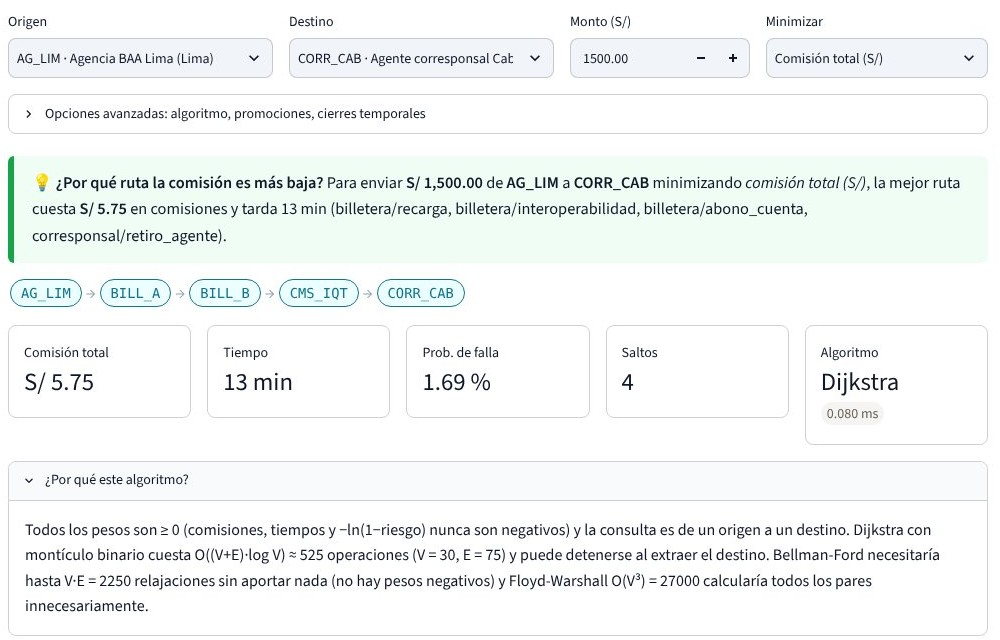
\includegraphics[width=\linewidth]{figs/cap_ruta.jpg}\\[-1pt]{\footnotesize (a)}
\end{minipage}\hfill
\begin{minipage}[b]{0.33\textwidth}\centering
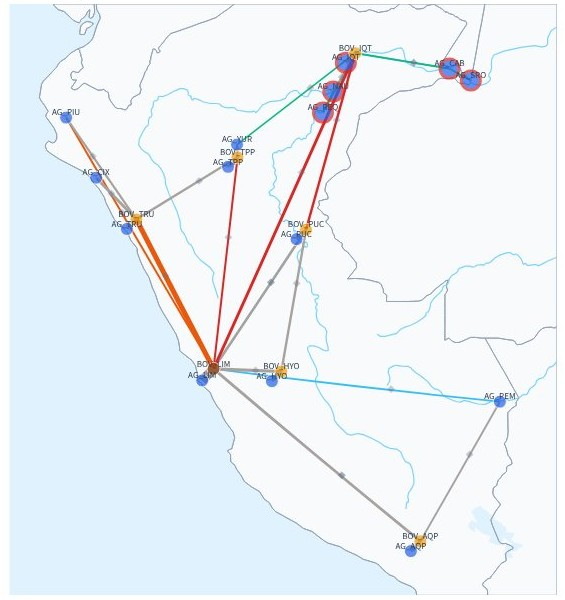
\includegraphics[width=\linewidth]{figs/cap_liquidez.jpg}\\[-1pt]{\footnotesize (b)}
\end{minipage}
\end{figure}

\subsection{Verificación}
Se ejecutaron 24 casos de prueba integrales, cada uno con entrada, condición inicial, resultado esperado y resultado
obtenido: 4 del Módulo~1 (carga, validación de 5 errores intencionales, alta y baja, consistencia), 7 del Módulo~2,
6 del Módulo~3, 5 del Módulo~4 y 2 del Módulo~5. Los 24 se superaron. Uno de ellos es el contraejemplo que justifica
la elección: en la red $S\!\to\!A$ (2), $S\!\to\!B$ (3), $B\!\to\!A$ ($-2$), Dijkstra devuelve 2 y Bellman-Ford
devuelve el valor correcto, 1. Además, 38 pruebas automatizadas con \id{pytest} cubren los cinco módulos, y la
comparación con NetworkX \citep{hagberg2008}, una biblioteca usada solo como referencia, coincidió en 30 de 30 redes
aleatorias para cada uno de los nueve algoritmos verificados.

%==================== 7. COMPLEJIDAD ====================
\section{Análisis de complejidad teórica y empírica}

Las mediciones se realizaron con \id{time.perf\_counter} (mejor de tres repeticiones) y \id{tracemalloc}, sobre
redes sintéticas de grado medio 3–4, en un equipo con procesador Intel Xeon de 2.1~GHz (2 núcleos), 8~GB de RAM y
Python~3.13. El exponente empírico $k$ se estimó por regresión de $\log t$ sobre $\log n$
(Tabla~\ref{tab:complejidad}, Figura~\ref{fig:bench}).
Los resultados confirman las decisiones. Floyd-Warshall crece con pendiente 3 y, con 200 nodos, tarda 450 veces más
que Dijkstra. Bellman-Ford es más lento que Dijkstra en todos los tamaños, pese a su parada temprana. Dinic supera a
Edmonds-Karp por un orden de magnitud y su ventaja crece con $n$. Tarjan es entre 1.1 y 1.4 veces más rápido que
Kosaraju. En las redes reales del proyecto, todos los análisis responden en milisegundos, lo que permite recalcular
al instante cada cierre de sucursal o cambio de escenario.

\begin{table}[!t]
\caption{Complejidad teórica frente a la empírica}\label{tab:complejidad}
\centering\small
\begin{tabularx}{\textwidth}{|L{2.6cm}|C{2.7cm}|C{1.55cm}|Y|}
\hline
\cab{Algoritmo} & \cab{Teórica (tiempo)} & \cab{$k$ empírico} & \cab{Medición representativa}\\ \hline
Dijkstra & $O((V+E)\log V)$ & 1.15 & 6.7 ms y 329 KB con $n=1\,600$\\ \hline
Bellman-Ford & $O(VE)$ & 1.09 & 4.8 ms con $n=800$ (parada temprana)\\ \hline
Floyd-Warshall & $O(V^3)$ & 3.13 & 271 ms y 1.6 MB ya con $n=200$\\ \hline
Edmonds-Karp & $O(VE^2)$ & 2.10 & 905 ms con $n=1\,600$\\ \hline
Dinic & $O(V^2E)$ & 1.30 & 22.6 ms con $n=1\,600$ (40 veces más rápido)\\ \hline
BFS / DFS & $O(V+E)$ & 1.26 / 1.23 & 53 ms con $n=16\,000$\\ \hline
Tarjan / Kosaraju & $O(V+E)$ & 1.22 / 1.29 & 87 ms frente a 116 ms con $n=16\,000$\\ \hline
Kruskal / Prim & $O(E\log E)$ / $O(E\log V)$ & 1.28 / 1.27 & 162 ms frente a 258 ms con $n=16\,000$\\ \hline
\end{tabularx}
\nota{Floyd-Warshall se midió hasta $n=200$ y Bellman-Ford hasta $n=800$ por su crecimiento. Los exponentes
algo mayores que 1 en los algoritmos lineales se deben al costo creciente de las estructuras de Python (diccionarios
y listas) y a la memoria caché.}
\end{table}

\begin{figure}[!t]
\caption{Tiempo de ejecución según el tamaño de la red (escala logarítmica)}\label{fig:bench}
\centering
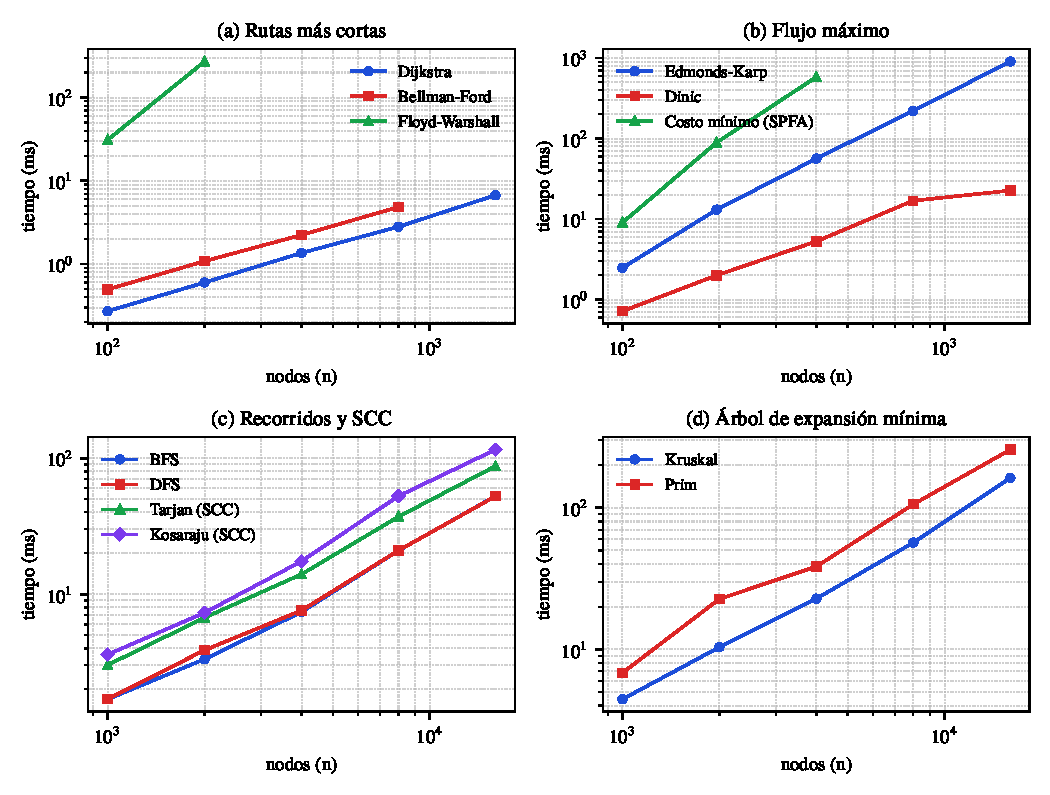
\includegraphics[width=0.74\textwidth]{figs/benchmarks.pdf}
\end{figure}

%==================== 8. DISCUSIÓN ====================
\section{Limitaciones y mejoras}
Los datos son simulados: tarifas, capacidades y patrones son plausibles pero no reales, y los umbrales de
detección deberían calibrarse con datos históricos. Como mejoras se proponen: aprendizaje estadístico sobre
características del grafo y detección incremental en tiempo real; sustituir SPFA por Dijkstra con potenciales de
Johnson en el flujo de costo mínimo; un reparto máximo-mínimo progresivo en lugar de una sola fracción $\lambda$;
y una planificación de liquidez de varios periodos con inventarios en bóveda.

%==================== 9. CONCLUSIONES ====================
\section{Conclusiones}
\subsection{Conclusión general}
Se desarrolló un sistema modular que modela la red de una entidad financiera con una estructura de grafo común y
resuelve los tres escenarios operativos con el algoritmo adecuado para cada uno. La validación con resultados
esperados, con algoritmos alternativos, con una biblioteca de referencia y con mediciones empíricas demuestra que la
selección algorítmica no es arbitraria: cada problema tiene una naturaleza distinta (conectividad, costo mínimo o
capacidad), y esa naturaleza determina el algoritmo óptimo y excluye a los demás.

\subsection{Conclusiones específicas}
\begin{enumerate}[label=CE\arabic*.,leftmargin=3.2em]
  \item La \textbf{lista de adyacencia} con soporte de multigrafo y cierre lógico es la estructura adecuada para redes
        financieras dispersas (densidad menor a 0.09): usa memoria $O(V+E)$ y permite simular mantenimientos sin
        reconstruir la red.
  \item En \textbf{fraude y lavado}, BFS, Tarjan y DFS acotada detectaron los cinco patrones plantados sin falsos
        positivos de riesgo alto o medio. No se usa un algoritmo de rutas más cortas ni de flujo porque el problema es
        de estructura y conectividad, no de costo o capacidad. Restringir la búsqueda de ciclos a las SCC hace
        abordable un problema exponencial.
  \item En \textbf{enrutamiento}, Dijkstra es el algoritmo óptimo porque todos los pesos son no negativos y la
        consulta es puntual. Bellman-Ford solo se justifica con bonificaciones negativas, y entonces detecta
        promociones explotables. Floyd-Warshall solo se justifica para la matriz de todos los pares. La ruta más
        barata depende del monto por los límites de cada canal.
  \item En \textbf{liquidez}, el problema es de capacidad. Dinic obtiene el flujo máximo 40 veces más rápido que
        Edmonds-Karp con 1\,600 nodos. El corte mínimo señala dónde invertir (el vuelo Lima–Iquitos). El MST no sirve
        para distribuir porque ignora capacidades y demandas. La política equitativa evita dejar agencias de la
        triple frontera sin efectivo a cambio de un sobrecosto de 3.0\,\%.
  \item El análisis \textbf{empírico} reprodujo el orden de la complejidad teórica (exponentes de 1.1 a 1.3 para los
        algoritmos casi lineales y de 3.1 para Floyd-Warshall), y los 24 casos de prueba y las 38 pruebas
        automatizadas se superaron.
\end{enumerate}

%==================== REFERENCIAS (APA 7) ====================
\renewcommand{\refname}{Referencias}
{\setstretch{1.0}\small
\addcontentsline{toc}{section}{Referencias}
\begin{thebibliography}{99}
\bibitem[Ahuja et~al.(1993)]{ahuja1993} Ahuja, R. K., Magnanti, T. L., \& Orlin, J. B. (1993). \textit{Network flows: Theory, algorithms, and applications}. Prentice Hall.
\bibitem[Banco Central de Reserva del Perú(2025)]{bcrp2025interop} Banco Central de Reserva del Perú. (2025). \textit{Estrategia de interoperabilidad de los pagos minoristas en Perú: Principales avances al primer semestre del 2025}. \url{https://www.bcrp.gob.pe/docs/Sistema-Pagos/articulos/estrategia-de-interoperabilidad-2025-1.pdf}
\bibitem[Bellman(1958)]{bellman1958} Bellman, R. (1958). On a routing problem. \textit{Quarterly of Applied Mathematics, 16}(1), 87--90. \url{https://doi.org/10.1090/qam/102435}
\bibitem[Cormen et~al.(2022)]{cormen2022} Cormen, T. H., Leiserson, C. E., Rivest, R. L., \& Stein, C. (2022). \textit{Introduction to algorithms} (4.ª ed.). MIT Press.
\bibitem[Dijkstra(1959)]{dijkstra1959} Dijkstra, E. W. (1959). A note on two problems in connexion with graphs. \textit{Numerische Mathematik, 1}(1), 269--271. \url{https://doi.org/10.1007/BF01386390}
\bibitem[Dinic(1970)]{dinic1970} Dinic, E. A. (1970). Algorithm for solution of a problem of maximum flow in networks with power estimation. \textit{Soviet Mathematics Doklady, 11}, 1277--1280.
\bibitem[Edmonds y Karp(1972)]{edmonds1972} Edmonds, J., \& Karp, R. M. (1972). Theoretical improvements in algorithmic efficiency for network flow problems. \textit{Journal of the ACM, 19}(2), 248--264. \url{https://doi.org/10.1145/321694.321699}
\bibitem[Hagberg et~al.(2008)]{hagberg2008} Hagberg, A. A., Schult, D. A., \& Swart, P. J. (2008). Exploring network structure, dynamics, and function using NetworkX. En G. Varoquaux, T. Vaught y J. Millman (Eds.), \textit{Proceedings of the 7th Python in Science Conference} (pp. 11--15).
\bibitem[Rojas Pedraza(2026)]{rojas2026guia} Rojas Pedraza, K. C. (2026). \textit{Proyecto II – Sistema de análisis y optimización de redes financieras} [Guía del proyecto, curso Programación III]. Universidad Nacional de San Antonio Abad del Cusco.
\bibitem[Superintendencia de Banca, Seguros y AFP(2025)]{sbs2025ambiental} Superintendencia de Banca, Seguros y AFP. (2025, 31 de octubre). \textit{SPLA: El lavado de activos proveniente de delitos ambientales está en aumento en el Perú} [Nota de prensa]. \url{https://www.sbs.gob.pe/noticia/detallenoticia/idnoticia/3882}
\bibitem[Superintendencia de Banca, Seguros y AFP(2026)]{sbs2026spla} Superintendencia de Banca, Seguros y AFP. (2026, 26 de octubre). \textit{Primera jornada de la SPLA 2026 resalta el rol de las instituciones y la inteligencia artificial frente al lavado de activos} [Nota de prensa]. \url{https://www.sbs.gob.pe/Noticia/DetalleNoticia?IdNoticia=4023}
\bibitem[Tarjan(1972)]{tarjan1972} Tarjan, R. (1972). Depth-first search and linear graph algorithms. \textit{SIAM Journal on Computing, 1}(2), 146--160. \url{https://doi.org/10.1137/0201010}
\bibitem[Yen(1971)]{yen1971} Yen, J. Y. (1971). Finding the \textit{k} shortest loopless paths in a network. \textit{Management Science, 17}(11), 712--716. \url{https://doi.org/10.1287/mnsc.17.11.712}
\end{thebibliography}}

\end{document}
